\section{PWM}

\begin{center}
    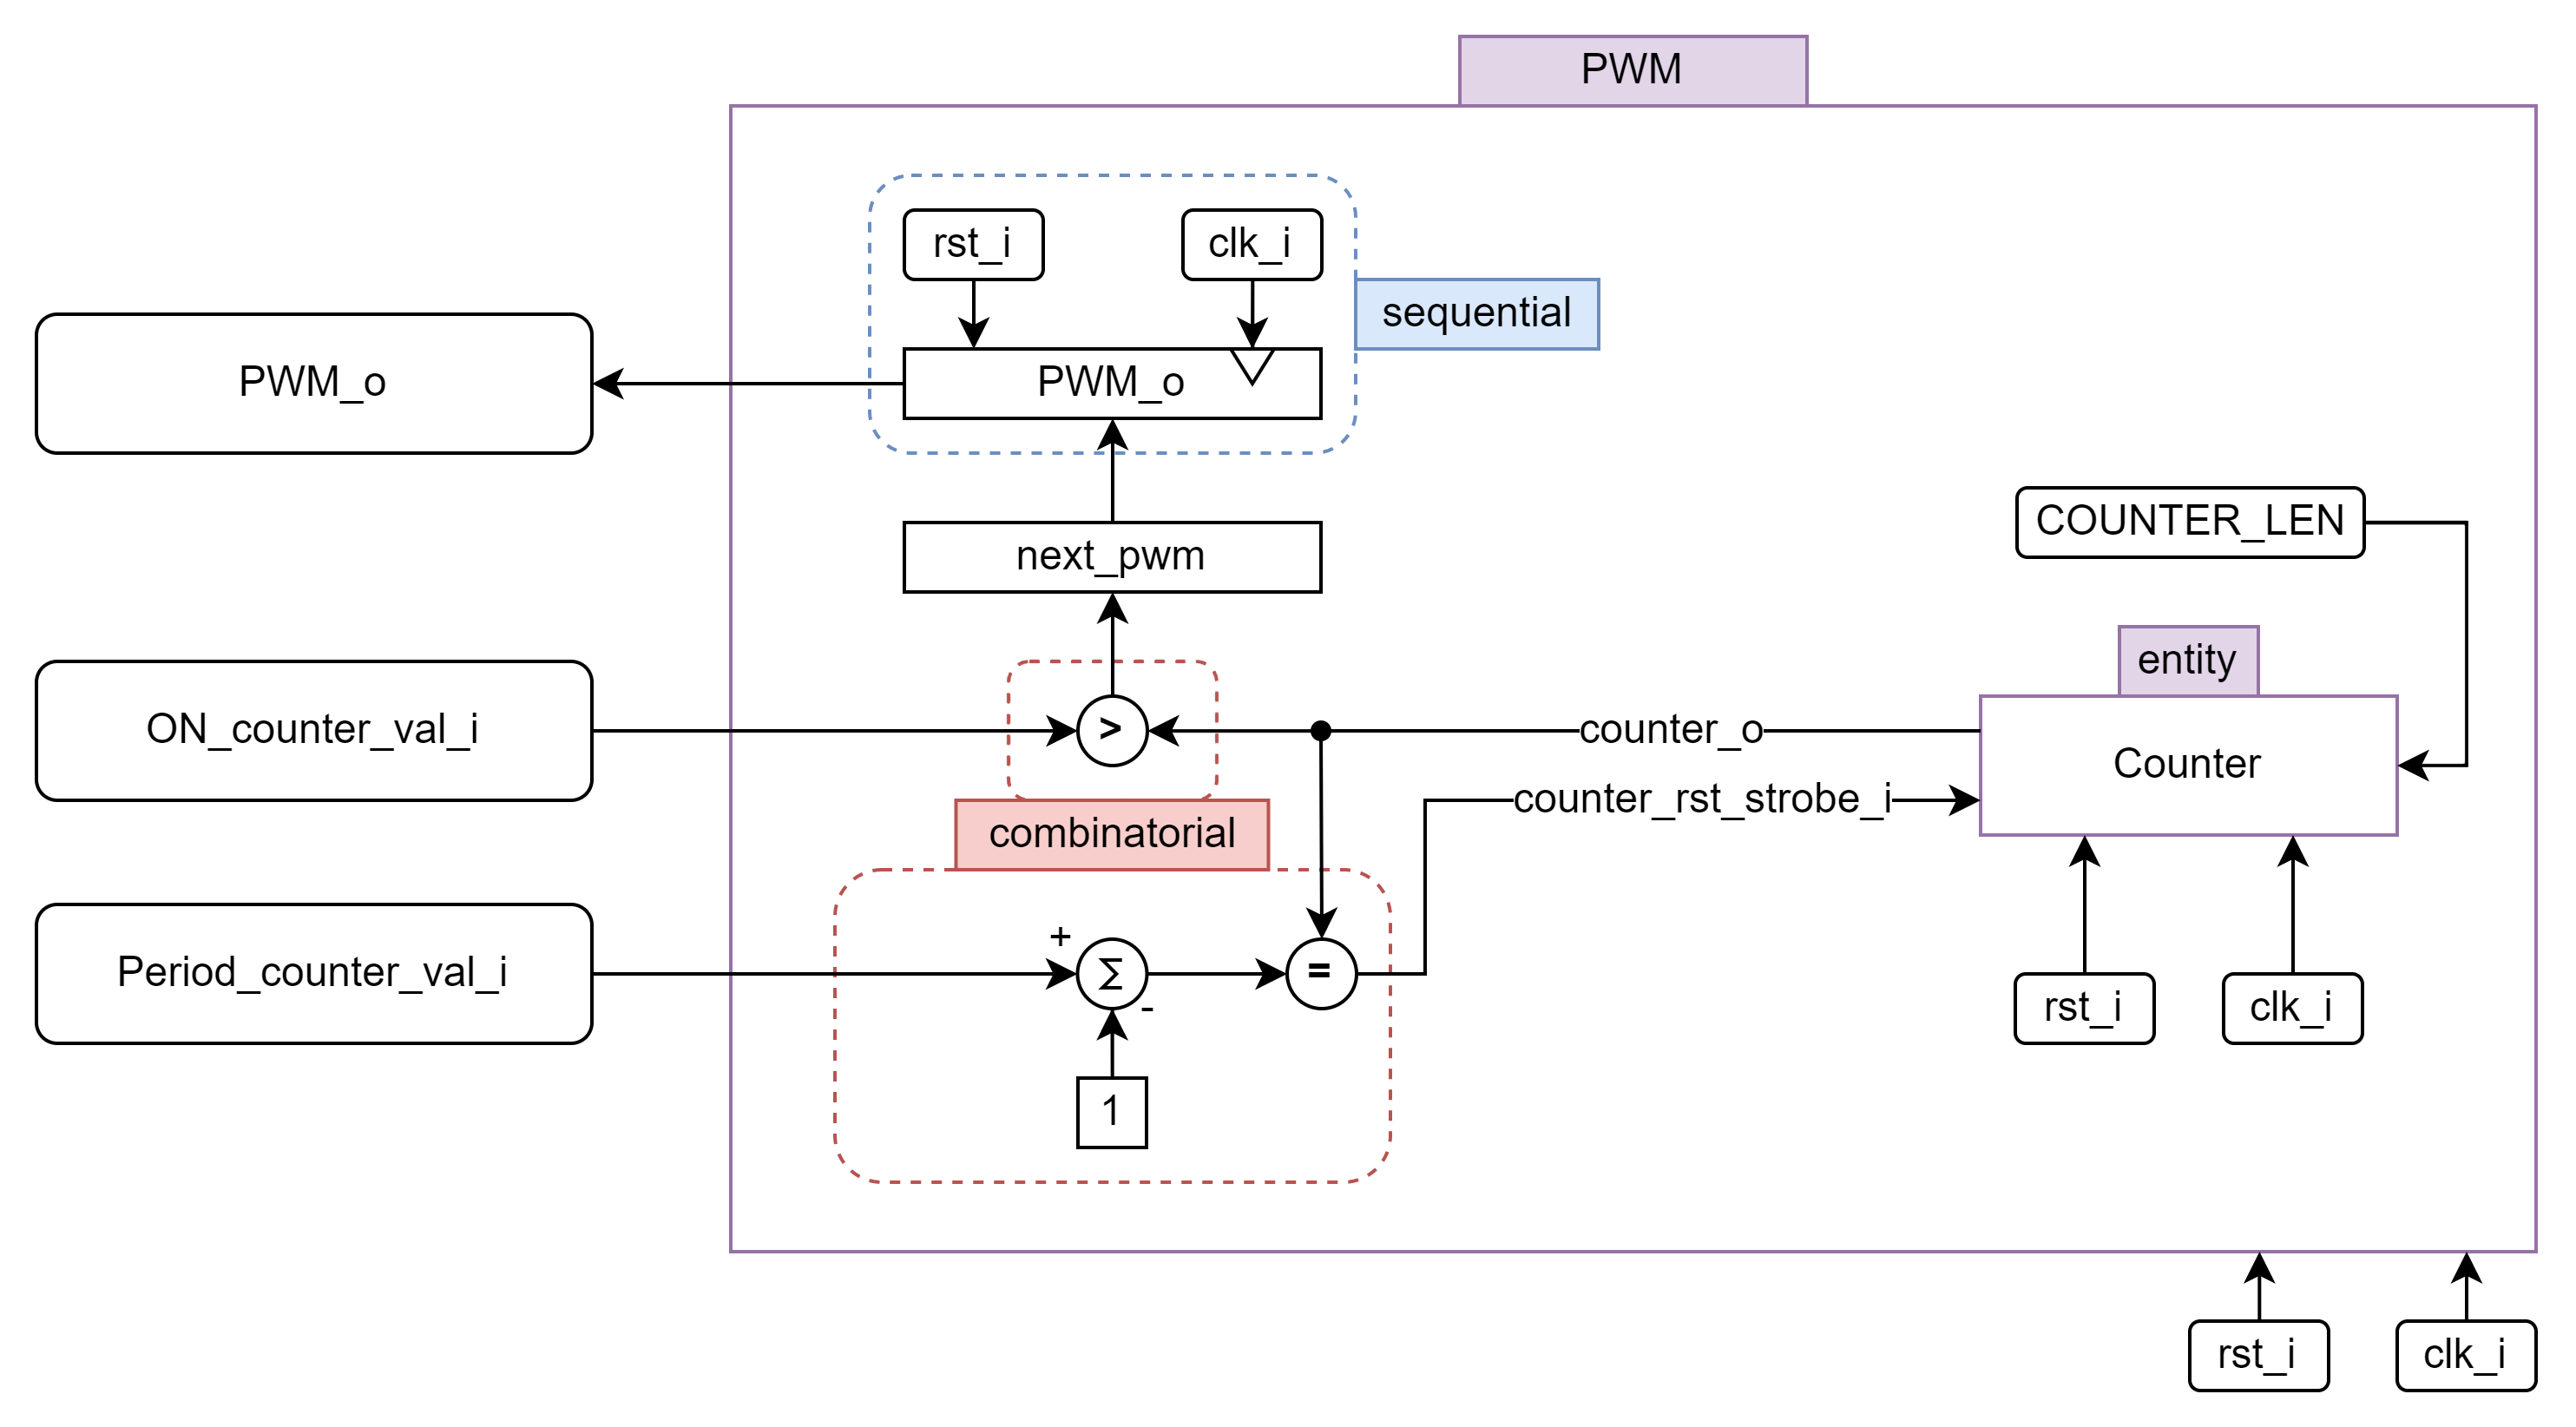
\includegraphics[width=1\linewidth]{images/2_PWM.png}
\end{center}

\textbf{Entity}\hrulefill

% \input{code/pwm_e}

\textbf{Architecture}\hrulefill

Dei Architektur des PWM-Generators besteht aus einem \lstinline{couner}-Entity und drei Prozessen.

Signale:

\begin{lstlisting}
    signal count            : unsigned(COUNTER_LEN-1 downto 0);
    signal count_reset_flag : std_ulogic := '0';
    signal next_pwm         : std_ulogic;
\end{lstlisting}

\newpage

(1) \lstinline{reg_seq : process (clk_i, rst_i)} 

\begin{quote}
    Der sequenzielle Prozess bestimmt das Clock- und Reset-Verhalten. Bei der
    steigenden Flanke wird dem PWM-Ausgang der kombinatorisch bestimmte nächste
    PWM-Zustand \lstinline{next_pwm} zugewiesen. Beim Reset wird der
    PWM-Ausgang auf \lstinline{'0'} gesetzt. 
\end{quote}

(2) \lstinline{pwm_comb : process (count, ON_counter_val_i)}

\begin{quote}
    Der kombinatorische Prozess setzt den nächsten PWM-Ausgangswert auf
    \lstinline{'1'}, falls der Counter-Wert des Counter-Entities die
    Duty-Cycle-Schwelle \lstinline{ON_counter_val_i} noch nicht erreicht hat.
    Wird dieser Wert überschritten, wird \lstinline{next_pwm} auf
    \lstinline{'0'} gesetzt.
\end{quote}

(3) \lstinline{clr_comb : process (count, Period_counter_val_i)}

\begin{quote}
    Dieser kombinatorische Prozess ist für das Zurücksetzen der Counters nach
    einer Periode zuständig. Dafür wird eine \lstinline{count_reset_flag},
    welche mit der Reset-Strobe des Counters verbunden ist, auf \lstinline{'1'}
    gesetzt. Somit wird im Counter-Entity ein synchroner Reset verursacht.
    Ansonsten ist die \lstinline{count_reset_flag} auf \lstinline{'0'}.
\end{quote}


\subsection*{Simulation}

\textbf{PWM-Test 1} \hrulefill

In dieser PWM-Testbench wird der PWM-Generator statisch, ohne veränderung des
Duty-Cycles betrachtet. Zu sehen ist hier die Konfiguration
\lstinline{Period_counter_val_i = 1111} (15) mit dem
Arbeitszyklus\newline \lstinline{ON_counter_val_i = 0110} (6). Da der im
Zyklus der Wert 0 mit gezählt wird muss bei einer Periode vom 15 also von 0 bis
14 gezählt werden. Nun ist zu sehen, dass der Duty-Cycle von 6 genau sechs
Pulse der PWM Periode high ist.

\begin{center}
    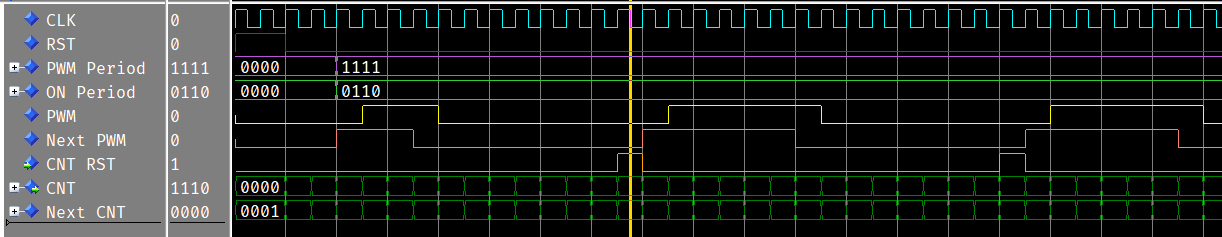
\includegraphics[width=1\linewidth]{images/SIM_PWM1.png}
\end{center}

\newpage
